\section{Diagrammi di sequenza}

	\subsection{Generazione Codice}
		Nel diagramma di seguenza di seguito è descritto il funzionamento di una richiesta di generazione di codice
		a partire da un progetto correttamente disegnato mediante l'applicazione.\\
		Arrivata la richiesta a index.js, file sul Server che si occupa di gestire le richieste del Client attraverso
		le funzioni di routing di Express.js.\\
		Express.js invia quindi una richiesta asincrona al Middleware che si occupa di richiedere, in maniera asincrona,
		ad un'istanza del servizio di parsing di effettuare l'operazione desiderata.\\
		Ogni ritorno avviene tramite callback fino a index.js che, nuovamente tramite Express.js, restituisce un template correttamente compilato
		in modo tale da poter essere utilizzato per la generazione del codice Java.
		\begin{figure}[h!]
			\centering
			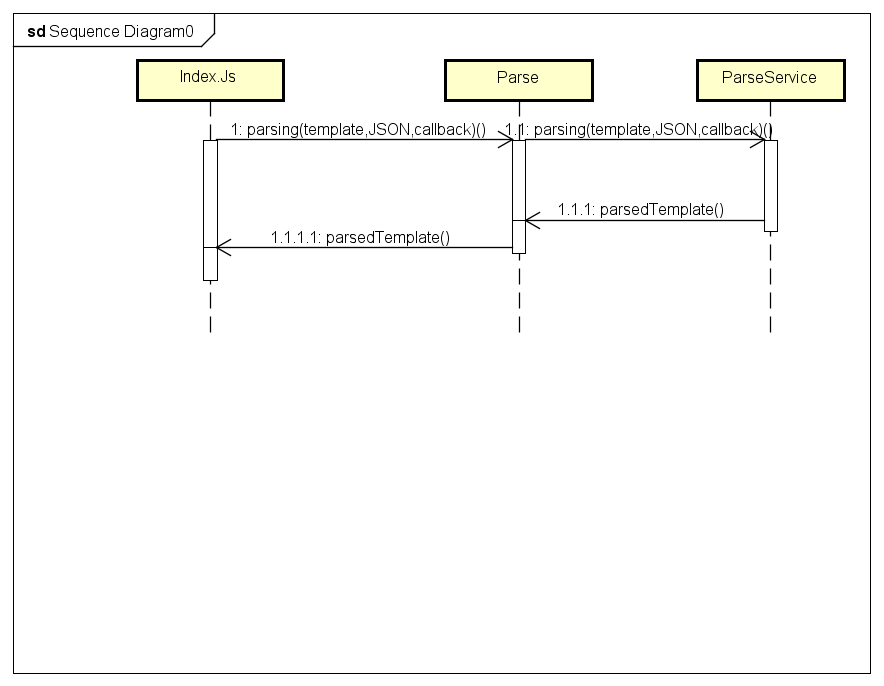
\includegraphics[scale=0.5]{Sequence/generazioneJava.png}
			\caption{Sequence diagram generazione codice java}
		\end{figure}

	\subsection{Caricamento moduli del Server}
		Nel diagramma di sequenza di seguito è descritto il funzionamento del caricamento di tutti i moduli del server che avviene, tipicamente,
		al primo avvio dell'applicativo.\\
		Quello che accade è una singola richiesta di Load() che si occupa di chiamare il ServerLoader che, tramite Express.js, effettua tutte
		le chiamate ai singoli loader dei vari moduli.\\
		Oltre all'istanza dei vari moduli presenti sul Server, vengono anche generate ed istanziate le chiavi crittografiche per la corretta gestione dei servizi di
		encrypt e decrypt.\\
		Ultimo, ma non meno importante, è la renderizzazione del template di Moustache necessario al parsing e alla generazione del codice Java così da avere sempre a dispozione
		un template renderizzato, quindi utilizzare da Moustache, ogni volta che viene richiesta la generazione di codice.\\
		\begin{figure}[h!]
			\centering
			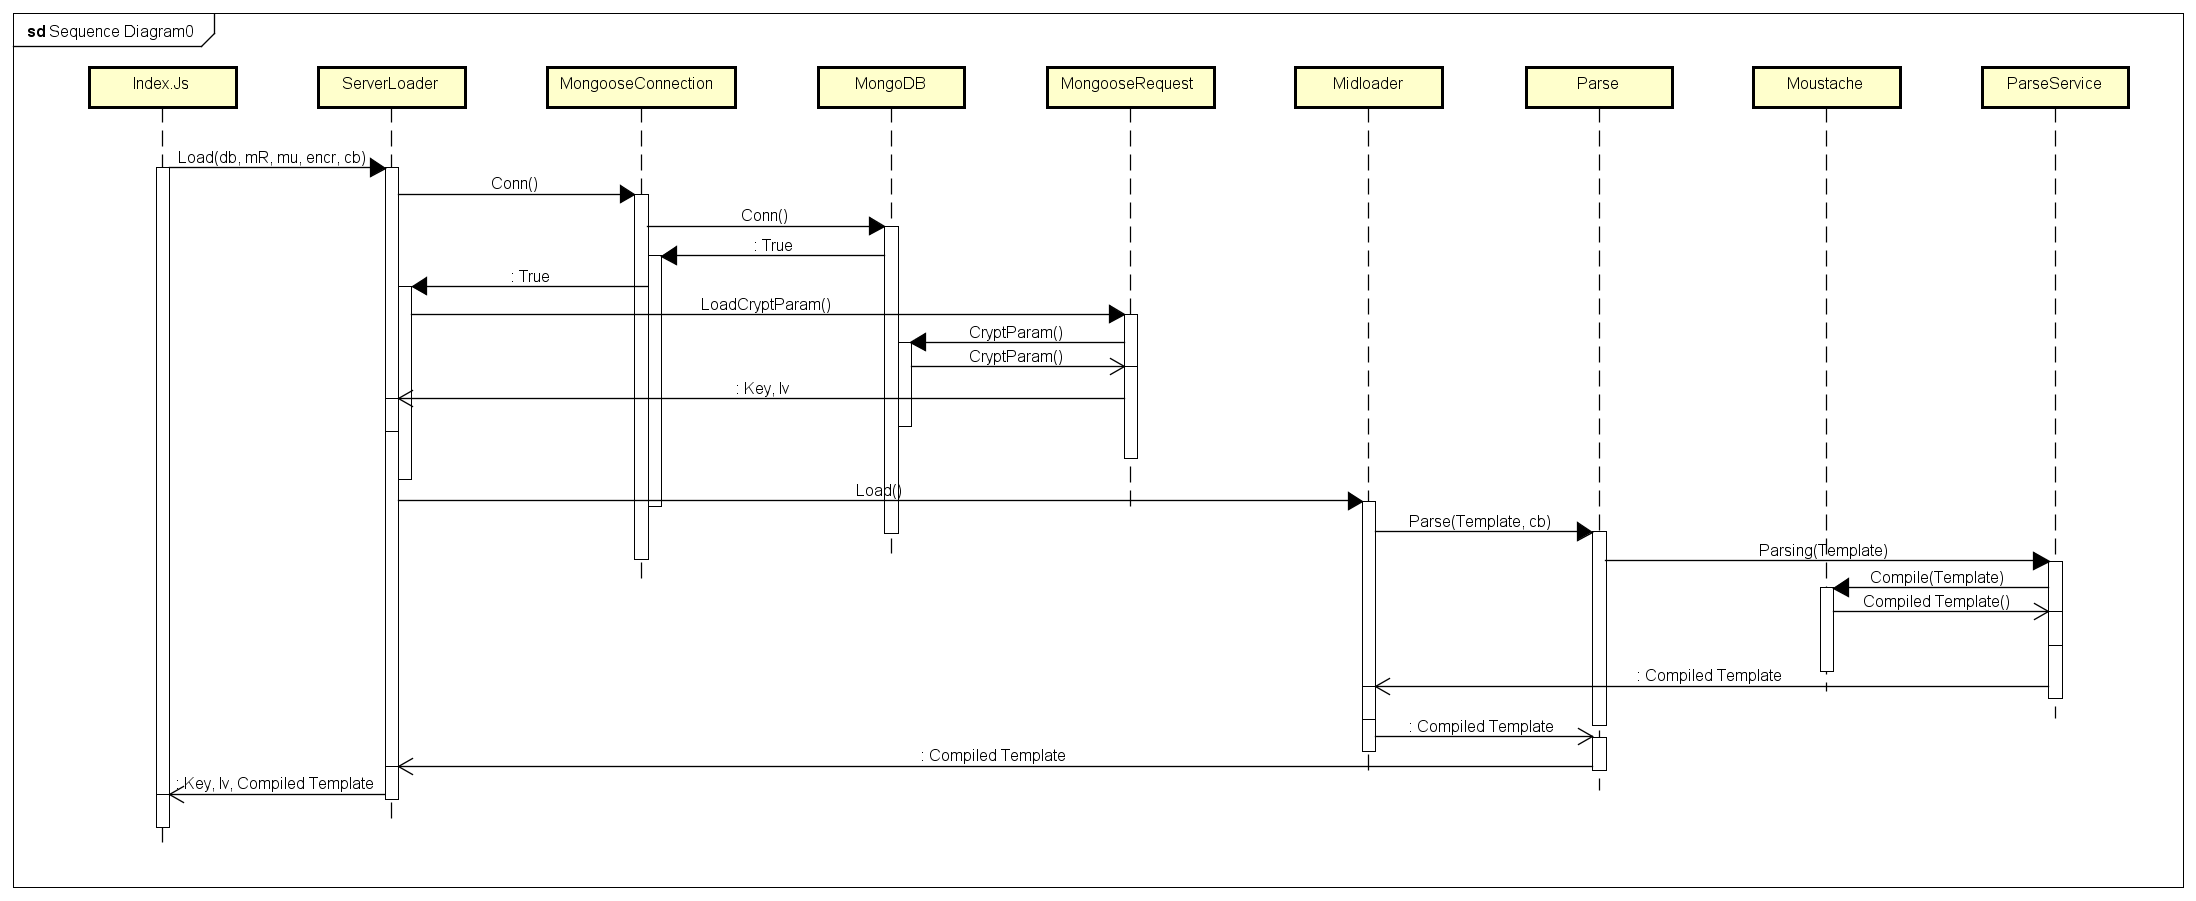
\includegraphics[scale=0.2]{Sequence/serverLoading.png}
			\caption{Sequence diagram caricamento moduli server}
		\end{figure}

		\subsection{Encrypt/Decrypt}
		Il diagramma di seguito mostra il funzionamento dei servizi di Encrypt e Decrypt.\\
		Quello che accade è che Index.js, sempre tramite il routing di Express.js, effettua una richiesta di encrypting (o decrypting) al Middleware desiderato il quale,
		effettuerà una richiesta ad un'istanza del servizio desiderato.\\
		Questo, tramite Forge, ritornerà semplicemente i file criptati o decriptati (a seconda della richiesta) al chiamante che gestirà
		il ritorno dell'informazione al Client.\\ 			
		\begin{figure}[h!]
			\centering
			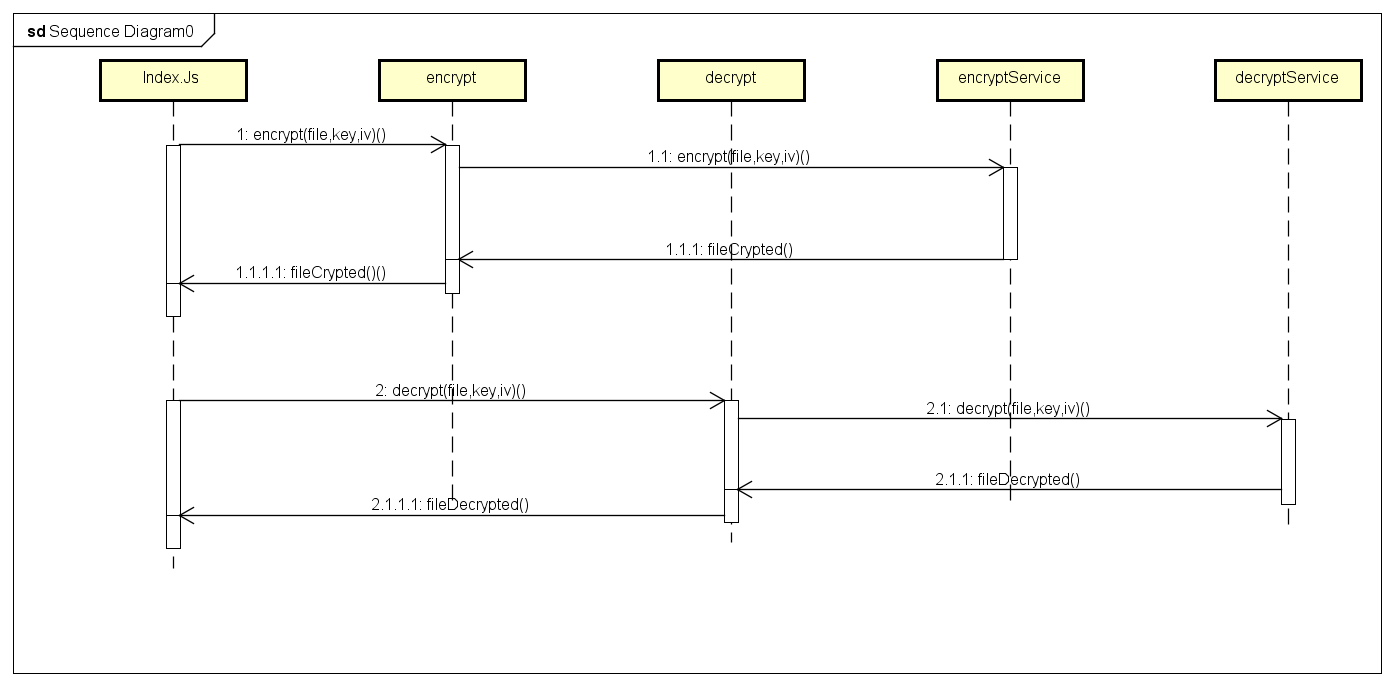
\includegraphics[scale=0.3]{Sequence/wncryptDecrypt.png}
			\caption{Sequence diagram per operazioni di encrypt e decrypt}
		\end{figure}
